% --- KHỐI 1: Đoạn văn dẫn đầu trang ---
\noindent
\hspace*{5.2cm}%
\begin{minipage}[t]{12.8cm}
    Hình 15 cho thấy rằng nếu chọn một giá trị $\varepsilon$ nhỏ hơn, thì có thể cần một giá trị $N$ lớn hơn.
\end{minipage}

\vspace{12pt}

% --- KHỐI 2: HÌNH 15 (Nhãn lề trái dóng chuẩn đáy trục đồ thị bên phải) ---
\noindent
\begin{minipage}[b]{4.4cm}
    \raggedright
    \textsf{\textbf{HÌNH 15}}\\[3pt]
    {\small $\displaystyle\lim_{x \to \infty} f(x) = L$}
    \vspace*{10pt}
\end{minipage}\hspace{0.8cm}%
\begin{minipage}[b]{12.8cm}
    \centering
    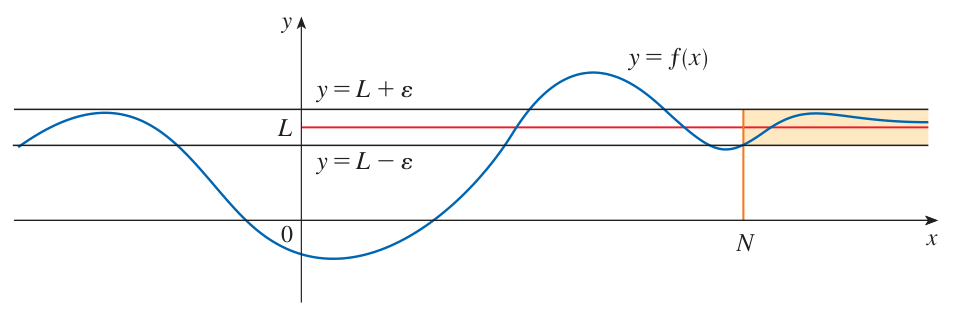
\includegraphics[width=0.88\linewidth]{images/p0170_fig1.png}
\end{minipage}

\vspace{16pt}

% --- KHỐI 3: Văn bản chuyển tiếp và Hộp Định nghĩa 8 ---
\noindent
\hspace*{5.2cm}%
\begin{minipage}[t]{12.8cm}
    Tương tự, một định nghĩa chính xác cho Định nghĩa 2 được đưa ra bởi Định nghĩa 8, được minh họa trong Hình 16.

    \vspace{6pt}
    \begin{tcolorbox}[
        colback=white,
        colframe=stewartred,
        arc=0mm,
        boxrule=0.8pt,
        left=8pt,
        right=8pt,
        top=7pt,
        bottom=7pt,
        boxsep=0pt
    ]
        \setlength{\abovedisplayskip}{5pt}%
        \setlength{\belowdisplayskip}{5pt}%
        \noindent
        \setlength{\fboxrule}{0.8pt}%
        \setlength{\fboxsep}{2pt}%
        \fcolorbox{stewartred}{white}{\textbf{\textsf{\color{stewartred}8}}}\hspace{0.6em}%
        \textbf{\textsf{\color{stewartred}Định nghĩa}}\hspace{0.8em}%
        Cho hàm số $f$ xác định trên khoảng $(-\infty, a)$ nào đó. Khi đó
        \[
            \lim_{x \to -\infty} f(x) = L
        \]
        có nghĩa là với mọi $\varepsilon > 0$ đều tồn tại một số $N$ tương ứng sao cho
        \[
            \text{nếu}\qquad x < N \qquad\text{thì}\qquad |f(x) - L| < \varepsilon
        \]
    \end{tcolorbox}
\end{minipage}

\vspace{16pt}

% --- KHỐI 4: HÌNH 16 (Dóng đáy nhãn lề với đồ thị) ---
\noindent
\begin{minipage}[b]{4.4cm}
    \raggedright
    \textsf{\textbf{HÌNH 16}}\\[3pt]
    {\small $\displaystyle\lim_{x \to -\infty} f(x) = L$}
    \vspace*{10pt}
\end{minipage}\hspace{0.8cm}%
\begin{minipage}[b]{12.8cm}
    \centering
    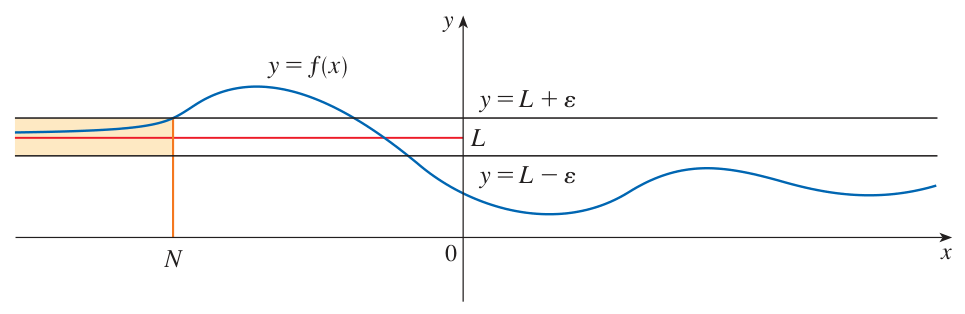
\includegraphics[width=0.88\linewidth]{images/p0170_fig2.png}
\end{minipage}

\vspace{18pt}

% --- KHỐI 5: Ví dụ 3 nhắc lại và VÍ DỤ 13 ---
\noindent
\hspace*{5.2cm}%
\begin{minipage}[t]{12.8cm}
    Trong Ví dụ 3, chúng ta đã tính được rằng
    \[
        \lim_{x \to \infty} \frac{3x^2 - x - 2}{5x^2 + 4x + 1} = \frac{3}{5}
    \]
    Trong ví dụ tiếp theo, chúng ta sử dụng máy tính bỏ túi (hoặc máy vi tính) để liên hệ khẳng định này với Định nghĩa 7 với $L = \frac{3}{5} = 0{,}6$ và $\varepsilon = 0{,}1$.

    \vspace{12pt}
    \noindent
    \textbf{\textsf{\color{stewartcyan}VÍ DỤ 13}}\hspace{0.8em}Sử dụng đồ thị để tìm một số $N$ sao cho
    \[
        \text{nếu}\qquad x > N \qquad\text{thì}\qquad \left| \frac{3x^2 - x - 2}{5x^2 + 4x + 1} - 0{,}6 \right| < 0{,}1
    \]
\end{minipage}
